\documentclass{article}
\usepackage{iclr_style}

\usepackage{graphicx}
\usepackage{array}
\usepackage{booktabs}
\usepackage{amsmath}
\usepackage{hyperref}
\usepackage{url}
\usepackage{xcolor}
\usepackage{listings}
\usepackage[numbers,sort&compress]{natbib}
\usepackage{tikz}
\usetikzlibrary{arrows.meta,positioning,shapes.geometric,fit,backgrounds}
\usepackage{placeins}

\hypersetup{
  colorlinks=true,
  linkcolor=black,
  citecolor=black,
  urlcolor=blue!50!black
}

% Compact listings for code snippets
\lstset{
  basicstyle=\ttfamily\scriptsize,
  breaklines=true,
  columns=fullflexible,
  keepspaces=true,
  showstringspaces=false,
  aboveskip=4pt,
  belowskip=4pt,
  xleftmargin=4pt,
  frame=single,
  framesep=2pt,
  rulecolor=\color{gray!40}
}

% Tighter caption spacing
\usepackage[font=small,skip=4pt]{caption}

\title{LLM-as-Judge as a Live Backend Evaluator: \\
A Product Prototype for Reliable Tool-Using Agents}

\author{Kevin Kwasnik \\ ECE 57000 --- Spring 2026 \\ Track 2: Product Prototype}

\date{}

\begin{document}
\maketitle

\begin{abstract}
Tool-using LLM agents are moving from demos into products, but the engineering question of how to know, automatically and after deployment, whether a given response is trustworthy remains largely unsolved. When an external tool fails, the agent often hallucinates a confident reply from the error context, and traditional observability captures the failure in traces without flagging the lie. This paper describes a product prototype in which LLM-as-Judge is promoted from an offline benchmark into a live backend evaluator wired into the application itself. The testbed is a grocery-shopping agent built on the Strands Agents SDK and grounded in the Kroger Product API, but the architecture is domain-agnostic: every agent and tool call is exported via OpenTelemetry to Arize Phoenix, and a session-exit evaluator pulls those spans back out, joins tool outputs onto their parent agent turns by \texttt{trace\_id}, and scores the agent's response against the \emph{actual tool output} rather than against its own self-report. This last design choice is the key contribution: by grounding the judge in the independently-captured tool trace, the evaluator sidesteps the self-bias concern that limits existing LLM-as-Judge tooling. On a five-day meal-plan query the agent produced a \$19.84 plan using only products present in the API context (faithfulness 1.00); on a run where the Kroger OAuth token had expired, the agent fabricated a confident shopping response despite a 401 error in the tool span, and the evaluator caught and scored it 0.00 without human inspection. Tool access is table stakes for grounded-agent products; the differentiator is an automated reliability signal wired in from day one.

\vspace{0.5em}
\noindent\textit{Code and LaTeX source:} \href{https://github.com/Kevin-Kwasnik/weekly-food-shopping}{\texttt{github.com/Kevin-Kwasnik/weekly-food-shopping}}
\end{abstract}

\section{Introduction}

\textbf{Target user.} The prototype targets the developer's own cohort: graduate students and early-career professionals who plan grocery trips weekly, cook most meals at home, and operate under tight financial and time budgets, typically \$50--\$80 per week for one to two people, with $\le$40 minutes of active cooking per meal. The project is an explicit case of the developer building for themselves as target user, with the limitation this implies (n=1 needs analysis) openly acknowledged. The motivation is a recurring personal pain: existing LLM assistants routinely produce recipes the developer cannot afford, cannot cook in the time available, or cannot actually buy at the specific Kroger location used each week.

\textbf{The real-world problem.} LLM meal planners exhibit four failure modes that make them unusable in this setting: (i) \emph{price hallucination}, confident dollar amounts untethered from any current catalog, causing plans to silently bust the budget; (ii) \emph{temporal blindness}, ``30-minute dinners'' that assume pre-chopped ingredients and a second cook; (iii) \emph{silent tool failures}, where an external API call errors but the agent continues as if it had succeeded, producing a response that looks grounded but is not; and (iv) \emph{no correctness signal}: the developer has no automated way to know, after shipping, whether a given response was faithful to the data it was supposed to use.

\textbf{User requirements.} Direct use of the prototype across iterative development surfaced five concrete success criteria: (R1) outputs must cite only products that actually exist at a named store at a named price; (R2) the total must respect a user-supplied budget ceiling; (R3) the plan must respect per-meal time limits and dietary constraints (e.g., non-spicy, high-protein); (R4) every agent response must be traceable, meaning inspectable after the fact to see which tool calls fired, what they returned, and how long they took; and (R5) the system must produce a machine-readable correctness score per response so regressions can be detected without human review.

Requirements R1--R3 are standard for a grounded shopping agent. R4 and R5, the shift in emphasis since Checkpoint~1, are what differentiate a demo from a product. Without them, the developer cannot tell whether a shipped change improved or silently degraded correctness.

\section{Related Work}

\textbf{Tool-augmented LLMs.} Grounding LLMs in external tools is the standard remedy for knowledge-cutoff and hallucination problems. The ReAct pattern~\citep{yao2023react} interleaves reasoning and tool calls, and is the conceptual basis for most modern agent SDKs including the one used here. For this prototype, the Strands Agents SDK~\citep{strands2025} was selected over LangChain and raw OpenAI function-calling for three reasons: (i) it exposes a minimal \texttt{@tool} decorator that keeps the Kroger wrapper readable; (ii) it emits OpenTelemetry spans natively, avoiding a separate instrumentation layer; and (iii) it is model-agnostic via the \texttt{OllamaModel} provider, enabling the use of a large open-weights model (\texttt{gpt-oss:120b-cloud}) without API lock-in.

\textbf{Observability for LLM agents.} Traditional APM tools (Datadog, New Relic) capture latency but not the LLM-specific span attributes (prompts, completions, tool arguments, retrieval context) that matter for debugging agent behavior. The OpenInference semantic convention~\citep{openinference2024} extends OTEL with these fields, and Arize Phoenix~\citep{arize2024phoenix} is its reference open-source collector. Phoenix was chosen over commercial alternatives (LangSmith, Braintrust) because it runs locally (\texttt{phoenix serve}, port 6006), requires no account, and exposes a Python client that returns spans as a DataFrame, which is critical for the evaluator.

\textbf{LLM-as-Judge and quality control of LLM output.} Automated correctness scoring by a stronger LLM has emerged as a practical alternative to expensive human evaluation. Zheng et al.~\citep{zheng2023judging} demonstrate that GPT-4 judges achieve over 80\% preference agreement with humans on MT-Bench, comparable to inter-human agreement, establishing LLM-as-Judge as a credible signal. Desmond et al.~\citep{desmond2024evalullm} build on this with EvaluLLM, a web tool that operationalizes LLM-as-Judge through pairwise comparison of generated outputs conditioned on user-defined criteria, and surface a key concern directly relevant to this project: LLM judges can exhibit bias toward self-generated outputs. Sandkuhl~\citep{sandkuhl2024quality} examines the broader question of whether an LLM can control the quality of LLM output, concluding that it can for consistency and completeness via triangulation and inverse mapping, but cannot fully substitute human judgment on relevance. The present project sits in this lineage: the judge scores faithfulness against the \emph{actual tool output} rather than the agent's self-report, which mitigates Desmond et al.'s self-bias concern because the judge compares two independent artifacts (the agent's response and the raw Kroger API response) rather than the agent's own claims.

\textbf{Grocery / retail APIs.} The Kroger Public API~\citep{krogerapi} was chosen over Instacart and Walmart alternatives because it is free for developer use, returns structured pricing per store location, and uses standard OAuth2 client-credentials; this matches the prototype's goal of a realistic engineering artifact rather than a screen-scraping hack.

\FloatBarrier
\section{Methodology}

The system has three loosely-coupled layers (Figure~\ref{fig:arch}), each owning a single responsibility.

\begin{figure}[!h]
\centering
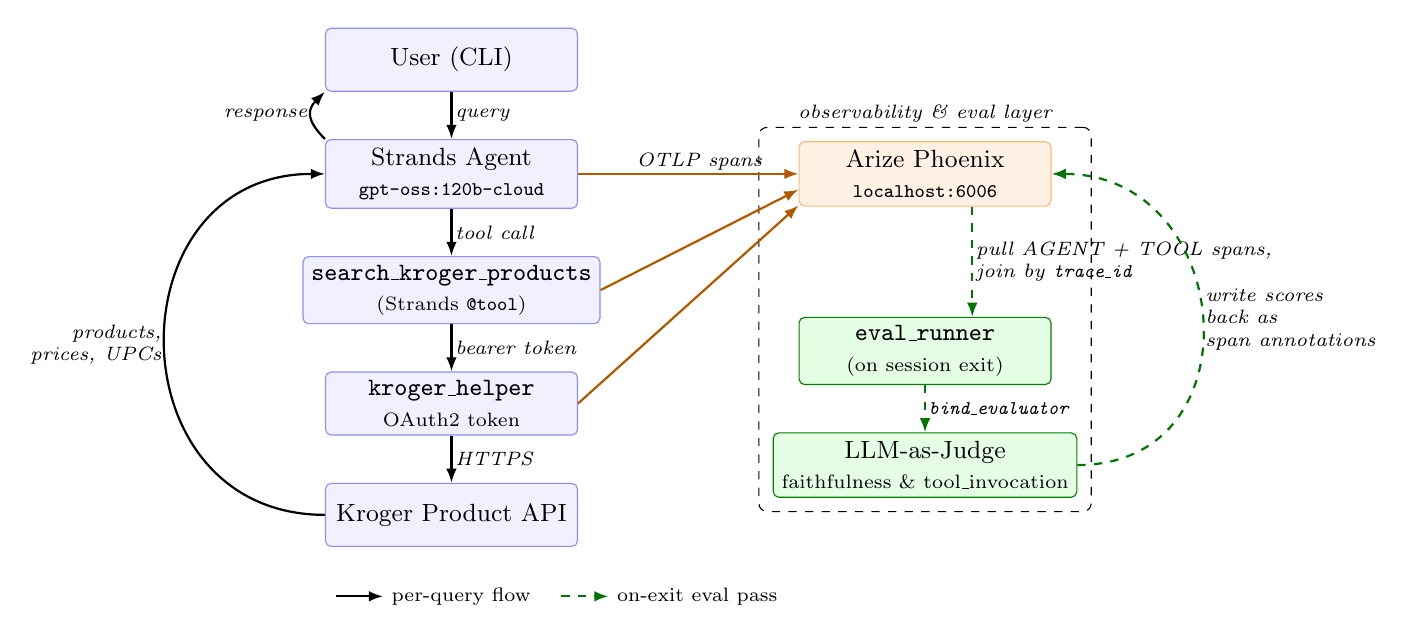
\begin{tikzpicture}[
    font=\small,
    node distance=6mm and 10mm,
    box/.style={draw, rounded corners=2pt, minimum height=8mm, minimum width=32mm, align=center, inner sep=3pt, fill=white},
    runtime/.style={box, fill=blue!6, draw=blue!45},
    obs/.style={box, fill=orange!10, draw=orange!55},
    eval/.style={box, fill=green!10, draw=green!50!black},
    arr/.style={-{Latex[length=1.8mm]}, thick},
    evalarr/.style={-{Latex[length=1.8mm]}, thick, dashed, draw=green!45!black},
    lbl/.style={font=\scriptsize\itshape, inner sep=1pt},
  ]

  % ===== LEFT COLUMN: runtime path (per-query) =====
  \node[runtime] (user)   {User (CLI)};
  \node[runtime, below=of user]  (agent)  {Strands Agent \\ \scriptsize \texttt{gpt-oss:120b-cloud}};
  \node[runtime, below=of agent] (tool)   {\texttt{search\_kroger\_products} \\ \scriptsize (Strands \texttt{@tool})};
  \node[runtime, below=of tool]  (oauth)  {\texttt{kroger\_helper} \\ \scriptsize OAuth2 token};
  \node[runtime, below=of oauth] (api)    {Kroger Product API};

  % Per-query arrows
  \draw[arr] (user)  -- node[lbl, right] {query} (agent);
  \draw[arr] (agent) -- node[lbl, right] {tool call} (tool);
  \draw[arr] (tool)  -- node[lbl, right] {bearer token} (oauth);
  \draw[arr] (oauth) -- node[lbl, right] {HTTPS} (api);

  % Return path (products / prices) — curved back up on the far left
  \draw[arr] (api.west) to[out=180, in=180, looseness=1.6]
      node[lbl, left, pos=0.5, align=right] {products, \\ prices, UPCs} (agent.west);
  \draw[arr] (agent.north west) to[out=135, in=225, looseness=1.4]
      node[lbl, left, pos=0.5] {response} (user.south west);

  % ===== RIGHT COLUMN: observability + eval =====
  \node[obs,  right=28mm of agent] (phoenix) {Arize Phoenix \\ \scriptsize \texttt{localhost:6006}};
  \node[eval, below=14mm of phoenix]        (evalrun) {\texttt{eval\_runner} \\ \scriptsize (on session exit)};
  \node[eval, below=of evalrun]             (judge)   {LLM-as-Judge \\ \scriptsize faithfulness \& tool\_invocation};

  % OTLP export: every runtime node sends spans to Phoenix
  \draw[arr, draw=orange!70!black]
      (agent.east)  -- node[lbl, above, pos=0.55] {OTLP spans} (phoenix.west);
  \draw[arr, draw=orange!70!black] (tool.east)   -- ([yshift=-2mm]phoenix.west);
  \draw[arr, draw=orange!70!black] (oauth.east)  -- ([yshift=-4mm]phoenix.west);

  % Eval pass (dashed, on exit)
  \draw[evalarr] ([xshift=6mm]phoenix.south) -- node[lbl, right, align=left] {pull AGENT + TOOL spans, \\ join by \texttt{trace\_id}} ([xshift=6mm]evalrun.north);
  \draw[evalarr] (evalrun) -- node[lbl, right] {\texttt{bind\_evaluator}} (judge);
  % Return the scores along the right edge of the eval column
  \draw[evalarr] (judge.east) to[out=0, in=0, looseness=1.6]
      node[lbl, right, pos=0.5, align=left] {write scores \\ back as \\ span annotations} (phoenix.east);

  % Legend (bottom)
  \begin{scope}[on background layer]
    \node[draw, dashed, rounded corners=3pt, inner sep=5pt,
          fit=(phoenix)(evalrun)(judge),
          label={[font=\scriptsize\itshape, yshift=-2pt]above:observability \& eval layer}] {};
  \end{scope}

  % Flow-type legend
  \node[font=\scriptsize, anchor=north west] at ([yshift=-4mm]api.south west)
      {\tikz\draw[arr] (0,0)--(6mm,0);~per-query flow \quad
       \tikz\draw[evalarr] (0,0)--(6mm,0);~on-exit eval pass};

\end{tikzpicture}
\caption{End-to-end system architecture. The runtime path (solid arrows, left) handles a single user query: the Strands Agent calls the Kroger tool, which fetches an OAuth2 token and hits the Product API; products flow back up to the agent and then to the user. In parallel, every agent and tool span is exported via OTLP to Arize Phoenix. At session exit, a separate eval runner (dashed arrows, right) pulls those spans back out, joins tool outputs onto their parent agent turns by \texttt{trace\_id}, scores the joined records with an LLM-as-Judge, and writes the scores back to Phoenix as span annotations. The eval loop never touches the hot path.}
\label{fig:arch}
\end{figure}

\textbf{Agent layer.} A Strands \texttt{Agent} wraps an \texttt{OllamaModel} pointed at \texttt{gpt-oss:120b-cloud} and is given one tool, \texttt{search\_kroger\_products}, plus a system prompt that enforces the user-constraint contract (budget, time, diet). The agent decides when to call the tool, with what search terms, and how to fold the returned products into its final answer. No retrieval-augmented generation (RAG) index is used; live API calls are cheap enough that caching was deferred.

\textbf{Tool layer.} \texttt{kroger\_products.py} exposes the Kroger \texttt{/products} endpoint via a Strands \texttt{@tool}-decorated function that accepts a store \texttt{location\_id} and a free-text \texttt{search\_term}. Authentication is handled by a separate helper (\texttt{kroger\_helper.py}) that performs the OAuth2 client-credentials flow and caches the bearer token. Structured output (product name, brand, size, unit price, UPC) is returned as JSON, which is exactly what the agent's grounding context needs.

\textbf{Observability and evaluation layer.} This is the architectural centerpiece. The OTEL \texttt{TracerProvider} is configured with an OpenInference span processor that reshapes Strands' native spans into the schema Phoenix expects, and a \texttt{BatchSpanProcessor} exports them over OTLP to the local Phoenix collector. At session exit, a separate evaluator pulls AGENT and TOOL spans back from Phoenix, joins tool outputs onto their parent agent turns by \texttt{trace\_id}, and scores the agent's output against that joined context using an LLM-as-Judge faithfulness evaluator (and a separate tool-invocation evaluator for the tool spans). Scores are written back to Phoenix as span annotations, so every trace in the UI carries its own correctness verdict.

\textbf{Why this split matters.} The three layers can fail independently, and the observability layer is designed to \emph{detect} failures in the other two. When the Kroger OAuth token expired during testing, the agent's final answer looked plausible --- but the tool span captured the 401 Unauthorized error, and the evaluator scored the agent's response as unfaithful because its claimed products were absent from the actual tool output (Section~\ref{sec:results}).

\FloatBarrier
\section{Implementation}

The full implementation lives in the attached repository. Two code excerpts capture the non-obvious engineering decisions.

\textbf{Tracing setup.} The tracing pipeline (\texttt{src/agent.py}, Listing~\ref{lst:trace}) has one subtle correctness issue that consumed significant debugging time: the Strands SDK initializes its own internal tracer on import, which causes every span to be exported \emph{twice} and corrupts the downstream eval data by double-counting. Setting \texttt{\_strands\_tracer.\_tracer\_instance = None} after importing the SDK is the fix; without it, faithfulness scores become meaningless because half the ``agent spans'' are duplicates with no tool children.

\begin{lstlisting}[caption={Tracing setup (abridged). The two non-obvious lines are the OpenInference span processor and the tracer-instance reset.},label=lst:trace,language=Python]
resource = Resource.create({
    "service.name": "grocery-assistant",
    "openinference.project.name": "weekly-shop",
})
provider = TracerProvider(resource=resource)
provider.add_span_processor(StrandsAgentsToOpenInferenceProcessor())
provider.add_span_processor(BatchSpanProcessor(
    OTLPSpanExporter(endpoint="http://localhost:6006/v1/traces")))
trace.set_tracer_provider(provider)

import strands.telemetry.tracer as _strands_tracer
_strands_tracer._tracer_instance = None   # prevent double-export
\end{lstlisting}

\textbf{Evaluator.} The evaluator (Listing~\ref{lst:eval}) is the component that makes the system a product rather than a demo. Phoenix separates AGENT-kind spans (a full LLM reasoning turn) from TOOL-kind spans (each API call), but correctness is only meaningful when they are joined: the agent's output must be scored against what the tool \emph{actually} returned, not against its own claims. Grouping tool outputs by \texttt{trace\_id} and merging them onto the parent agent span produces a \texttt{tool\_context} column that the \texttt{bind\_evaluator} call routes into the judge's \texttt{context} slot. The judge then sees the user query, the agent's answer, and the ground-truth API response, and scores faithfulness against that context.

\begin{lstlisting}[caption={Faithfulness evaluator (abridged). The groupby-and-merge step is what makes the judge's score meaningful.},label=lst:eval,language=Python]
client = Client(base_url="http://localhost:6006")
spans = client.spans.get_spans_dataframe(project_identifier="weekly-shop")
agent_spans = spans[spans['span_kind'] == 'AGENT'].copy()
tool_spans  = spans[spans['span_kind'] == 'TOOL'].copy()

tool_context = (tool_spans
    .groupby('context.trace_id')['attributes.output.value']
    .apply(lambda xs: "\n\n".join(str(x) for x in xs if x))
    .reset_index()
    .rename(columns={'attributes.output.value': 'tool_context'}))

agent_spans = agent_spans.merge(tool_context, on='context.trace_id', how='left')

bound = bind_evaluator(
    evaluator=correctness_eval,
    input_mapping={
        "input":   "attributes.input.value",
        "output":  "attributes.output.value",
        "context": "tool_context",   # <-- REAL tool output, not agent self-report
    })
\end{lstlisting}

The evaluator runs on session exit rather than inline, so it adds zero latency to user interactions. A second \texttt{tool\_invocation} evaluator runs on the TOOL spans themselves, checking whether the arguments passed to \texttt{search\_kroger\_products} were sensible given the user's query.

\FloatBarrier
\section{Experiment}
\label{sec:results}

The prototype was evaluated on four representative queries covering the success criteria from Section~1. Two runs (one success, one failure) are reported in detail below; both are visible in the attached Phoenix traces and eval dumps.

\begin{table}[!h]
\centering
\small
\caption{Representative evaluation runs. Faithfulness is scored against joined tool context; tool\_invocation is scored against the schema and the user's stated intent. All scores are produced by an LLM-as-Judge, not by the agent itself.}
\label{tab:results}
\begin{tabular}{@{}l>{\raggedright\arraybackslash}p{0.38\textwidth}cc>{\raggedright\arraybackslash}p{0.32\textwidth}@{}}
\toprule
\textbf{Span} & \textbf{Query / invocation (abridged)} & \textbf{Latency} & \textbf{Score} & \textbf{Judge rationale} \\
\midrule
agent & ``Inexpensive 5-day dinner plan, 2 people, 3 chicken / 2 pork nights at store 01400943'' & 37.9s & 1.00 (faithful) & Plan cites only products returned by the tool; totals match. \\
agent & ``Salads at 01400943'' (during OAuth 401) & 12.3s & 0.00 (unfaithful) & Generic salad taxonomy presented as if grounded; tool actually returned a 401 error. \\
tool & \texttt{search\_kroger\_products} with \texttt{search\_term=\,``bread''} & 1.4s & 1.00 (correct) & Schema-valid, sensible term. \\
tool & \texttt{search\_kroger\_products} with \texttt{search\_term=\,``eggs''} for ``5-day breakfast plan'' & 2.4s & 0.00 (incorrect) & Single-item search does not address multi-meal planning intent. \\
\bottomrule
\end{tabular}
\end{table}

\textbf{Successful grounded run.} Given the query \emph{``please create the most inexpensive dinner plan for 2, 5 days, using chicken 3 nights, and pork 2 nights at store 01400943''}, the agent called \texttt{search\_kroger\_products} for chicken, pork, and rice and returned a structured plan totalling \$19.84. Every product cited in the final answer (Heritage Farm\textregistered\ chicken breasts at \$2.69, Pork Bone-In Center Thick Cut Chops at \$4.79, Riceland Extra Long Grain White Rice at \$2.19) appeared verbatim in the tool span output. The judge explained: \emph{``All product names, prices, and quantities match the context, and the totals are accurate. There is no fabricated or misleading information.''} Faithfulness score: $\mathbf{1.00}$.

\textbf{Caught hallucination.} On an earlier run, the Kroger OAuth token request returned 401 Unauthorized. The tool span recorded the error cleanly --- not swallowed silently --- but the agent, seeing only an error string in its context, proceeded to generate a confident, formatted response with a generic taxonomy of salads and a parenthetical claim about the app showing ``every ready-to-eat salad currently stocked'' (implying live data access that did not exist). The faithfulness evaluator, which had access to the real tool output (the 401 error), scored this $\mathbf{0.00}$ and labelled it \emph{unfaithful}, with the explanation: \emph{``The response contradicts the context, as the context shows a clear authentication failure, making it impossible to pull such data. Therefore, the response contains unfaithful information.''} This is the exact failure mode that motivated the project, and the eval loop caught it without human inspection.

\textbf{Tool-invocation evaluator.} Two tool calls from a single ``affordable 5-day breakfast plan'' query illustrate why the tool-invocation score is a useful complement to faithfulness. A \texttt{search\_term=``bread''} invocation was scored \emph{correct} (schema-valid, realistic term), while \texttt{search\_term=``eggs''} for the same broader planning intent was scored \emph{incorrect} because a single-product search does not match the user's multi-item planning goal. These two scores together let the developer distinguish \emph{``the agent asked the tool the wrong question''} from \emph{``the tool answered correctly but the agent ignored it.''}

\textbf{Assessment against user requirements.} R1 (real products at real prices), R2 (budget respected), and R3 (constraints honored) are demonstrably met on the successful run. R4 (traceability) is met structurally, as every span is in Phoenix with input, output, timing, and tool arguments, and R5 (automated correctness signal) is met by the dual-evaluator setup, which is the contribution that lifts this project from Checkpoint~1's demo into a testable product.

\section{Discussion and Conclusion}

\textbf{What worked.} The separation of the observability layer from the agent itself was the single highest-leverage design decision. Because evaluation runs on stored spans rather than inline, the developer can swap the judge model, re-score historical runs, and A/B different system prompts without redeploying the agent. The OpenInference convention was essential here: it is the contract that lets a separate process understand the agent's traces.

\textbf{Limitations.} Four honest caveats. First, the evaluator and the agent both run on Ollama models, which introduces shared-bias risk despite the tool-context grounding; a meaningful next step is to run the judge on a different provider family. Second, faithfulness is a necessary but not sufficient correctness signal: a plan can be faithful to the tool output and still bust the budget if the agent mis-sums prices, so a dedicated budget-adherence evaluator is the natural follow-up. Third, the tool-invocation judge in the breakfast example arguably confuses \emph{tool selection} with \emph{tool invocation}, penalizing a schema-correct call for matching only part of the user's intent. The prompt for that evaluator needs tightening, or the project needs a third ``plan-completeness'' evaluator. Fourth, evaluation is currently ad-hoc on $\sim$4 queries; a held-out test set of 30--50 queries with human-labeled ground truth is needed before any claim of generalization.

\textbf{Next steps.} (i) Escalate tool errors to the agent so 401s trigger a user-facing ``the store system is down'' rather than a confident hallucination. (ii) Add a Pydantic-structured output schema (meal plan $\to$ day $\to$ recipe $\to$ ingredient $\to$ price) so the budget-adherence evaluator can score deterministically rather than via LLM judge. (iii) Move from CLI to a thin web UI with streaming status (``searching bread...'') to address the latency surfaced in Table~\ref{tab:results}. (iv) Build a labeled eval set and track the two scores as regression gates in CI.

\textbf{Conclusion and Track 2 contribution.} This work contributes a working product prototype (Track 2) that demonstrates a transferable architectural pattern: LLM-as-Judge promoted from an offline benchmark into a live backend evaluator, wired into the application via OpenTelemetry and grounded in independently-captured tool traces rather than in the agent's self-report. The prototype itself is a grocery-shopping agent built on Strands and the Kroger API, but the contribution is the evaluation architecture, which is domain-agnostic and reusable for any tool-using agent product. The empirical payoff is concrete: the same system that produced a faithful \$19.84 meal plan also caught its own confident hallucination during an OAuth failure, scoring it 0.00 without human inspection. Tool access is table stakes for grounded-agent products; the differentiator is an automated reliability signal wired in from day one.

% ICLR explicitly excludes references from the page count.
\newpage
\bibliographystyle{plainnat}
\begin{thebibliography}{9}

\bibitem[Yao et al.(2023)]{yao2023react}
S.~Yao, J.~Zhao, D.~Yu, N.~Du, I.~Shafran, K.~Narasimhan, and Y.~Cao.
\newblock ReAct: Synergizing Reasoning and Acting in Language Models.
\newblock \emph{ICLR}, 2023.
\newblock \url{https://doi.org/10.48550/arXiv.2210.03629}.

\bibitem[Zheng et al.(2023)]{zheng2023judging}
L.~Zheng, W.-L.~Chiang, Y.~Sheng, S.~Zhuang, Z.~Wu, Y.~Zhuang, Z.~Lin, Z.~Li, D.~Li, E.~P.~Xing, H.~Zhang, J.~E.~Gonzalez, and I.~Stoica.
\newblock Judging LLM-as-a-Judge with MT-Bench and Chatbot Arena.
\newblock \emph{Advances in Neural Information Processing Systems (NeurIPS) Datasets and Benchmarks Track}, 2023.
\newblock \url{https://doi.org/10.48550/arXiv.2306.05685}.

\bibitem[Desmond et al.(2024)]{desmond2024evalullm}
M.~Desmond, Z.~Ashktorab, Q.~Pan, J.~M.~Johnson, and C.~Dugan.
\newblock EvaluLLM: LLM Assisted Evaluation of Generative Outputs.
\newblock In \emph{Companion Proceedings of the 29th International Conference on Intelligent User Interfaces (IUI Companion '24)}, pages 30--32, 2024.
\newblock \url{https://doi.org/10.1145/3640544.3645216}.

\bibitem[Sandkuhl(2024)]{sandkuhl2024quality}
K.~Sandkuhl.
\newblock LLM-Assistance for Quality Control of LLM Output.
\newblock In \emph{Perspectives in Business Informatics Research (BIR 2024)}, LNBIP 529, pages 36--50. Springer, 2024.
\newblock \url{https://doi.org/10.1007/978-3-031-71333-0_3}.

\bibitem[Strands Agents(2025)]{strands2025}
Strands Agents.
\newblock Strands Agents SDK (open-source Python SDK, originally released by AWS).
\newblock \url{https://github.com/strands-agents/sdk-python}, 2025.

\bibitem[Arize AI(2024)]{arize2024phoenix}
Arize AI.
\newblock Arize Phoenix: Open-Source Observability for LLM Applications.
\newblock \url{https://github.com/Arize-ai/phoenix}, 2024.

\bibitem[Arize AI(2024)]{openinference2024}
Arize AI.
\newblock OpenInference Semantic Conventions for LLM Observability.
\newblock \url{https://github.com/Arize-ai/openinference}, 2024.

\bibitem[Kroger(2024)]{krogerapi}
The Kroger Co.
\newblock Kroger Developer Portal --- Product API v1.
\newblock \url{https://developer.kroger.com/documentation/api-products/public/products/overview}, 2024.

\end{thebibliography}

\section*{LLM Acknowledgments}

The author used Anthropic's Claude (Claude Opus 4.7, via claude.ai) during the preparation of this manuscript. The LLM's role was limited to writing assistance: drafting and revising prose, restructuring sections for clarity, and producing the LaTeX for the system-architecture figure and the results table. All technical decisions, system design choices, implementation, experimental runs, interpretation of evaluation results, and the core argument of the paper are the author's own. The author reviewed and edited all LLM-generated text and bears sole responsibility for the content of the final submission.

\end{document}
